\subsection{Genesis}

\begin{figure}[htb!]
  \centering
    \subfloat[]{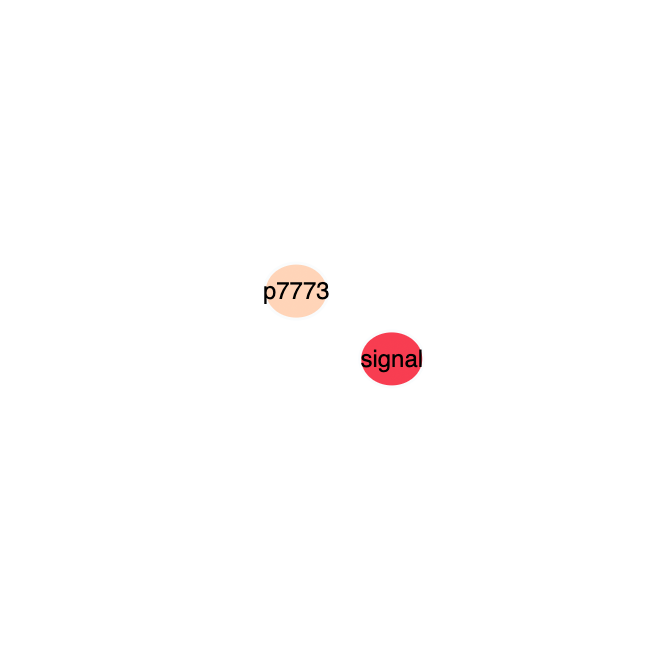
\includegraphics[width=0.33\textwidth]{graphics/analysis/mini-scenarios/become-router/1.png} \label{fig:filmstrips-genesis-a}}
    \subfloat[]{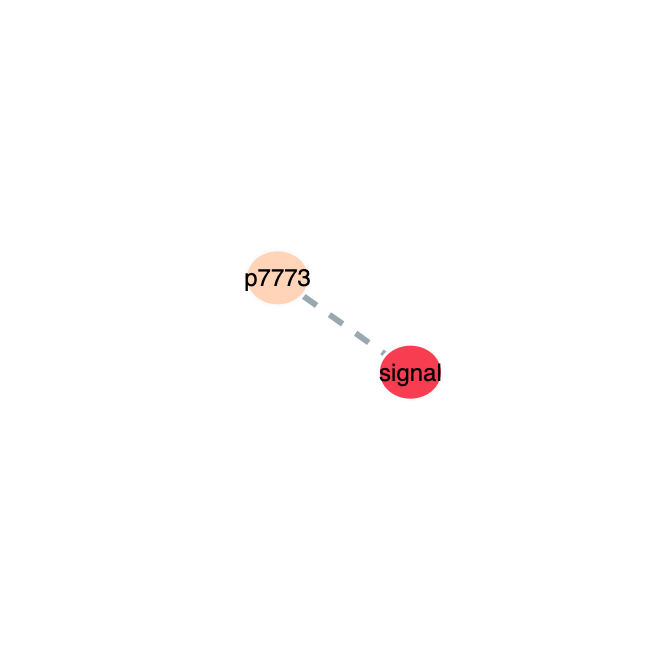
\includegraphics[width=0.33\textwidth]{graphics/analysis/mini-scenarios/become-router/2.png} \label{fig:filmstrips-genesis-b}}
	\subfloat[]{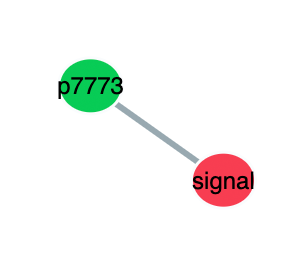
\includegraphics[width=0.33\textwidth]{graphics/analysis/mini-scenarios/become-router/3.png} \label{fig:filmstrips-genesis-c}}
	\caption{Join network as first peer}
\label{fig:filmstrips-genesis}
\end{figure}

The first scenario is called \textit{Genesis} because the very first peer is joining the network. The peer with the role \signal has to be present already, otherwise a network can not be created (\vref{fig:filmstrips-genesis-a}). 

A new peer has the role \newbie by default. Because of the \newbie role the peer has the desire to open a connection to the network entry point. Thus, it is opening a \glsfirst{ws} connection to the \signal peer (\vref{fig:filmstrips-genesis-b}). The address for the \gls{ws} connection is specified in the initial configuration of the peer.

After the connection has been established, the \signal is upgrading the role of the peer to the roles \router and \peer as it does not know another router (\vref{fig:filmstrips-genesis-c}). The role \peer is given to all peers that are joining the network.
Because of its new \router role, \lstinline{p7773} keeps the connection to the \signal alive.
